\presub
\subsection{The InterestSketch Framework}
\postsub
\label{sub:findinterest}
%
\begin{figure}[htbp]
	\centering
	\prefig
	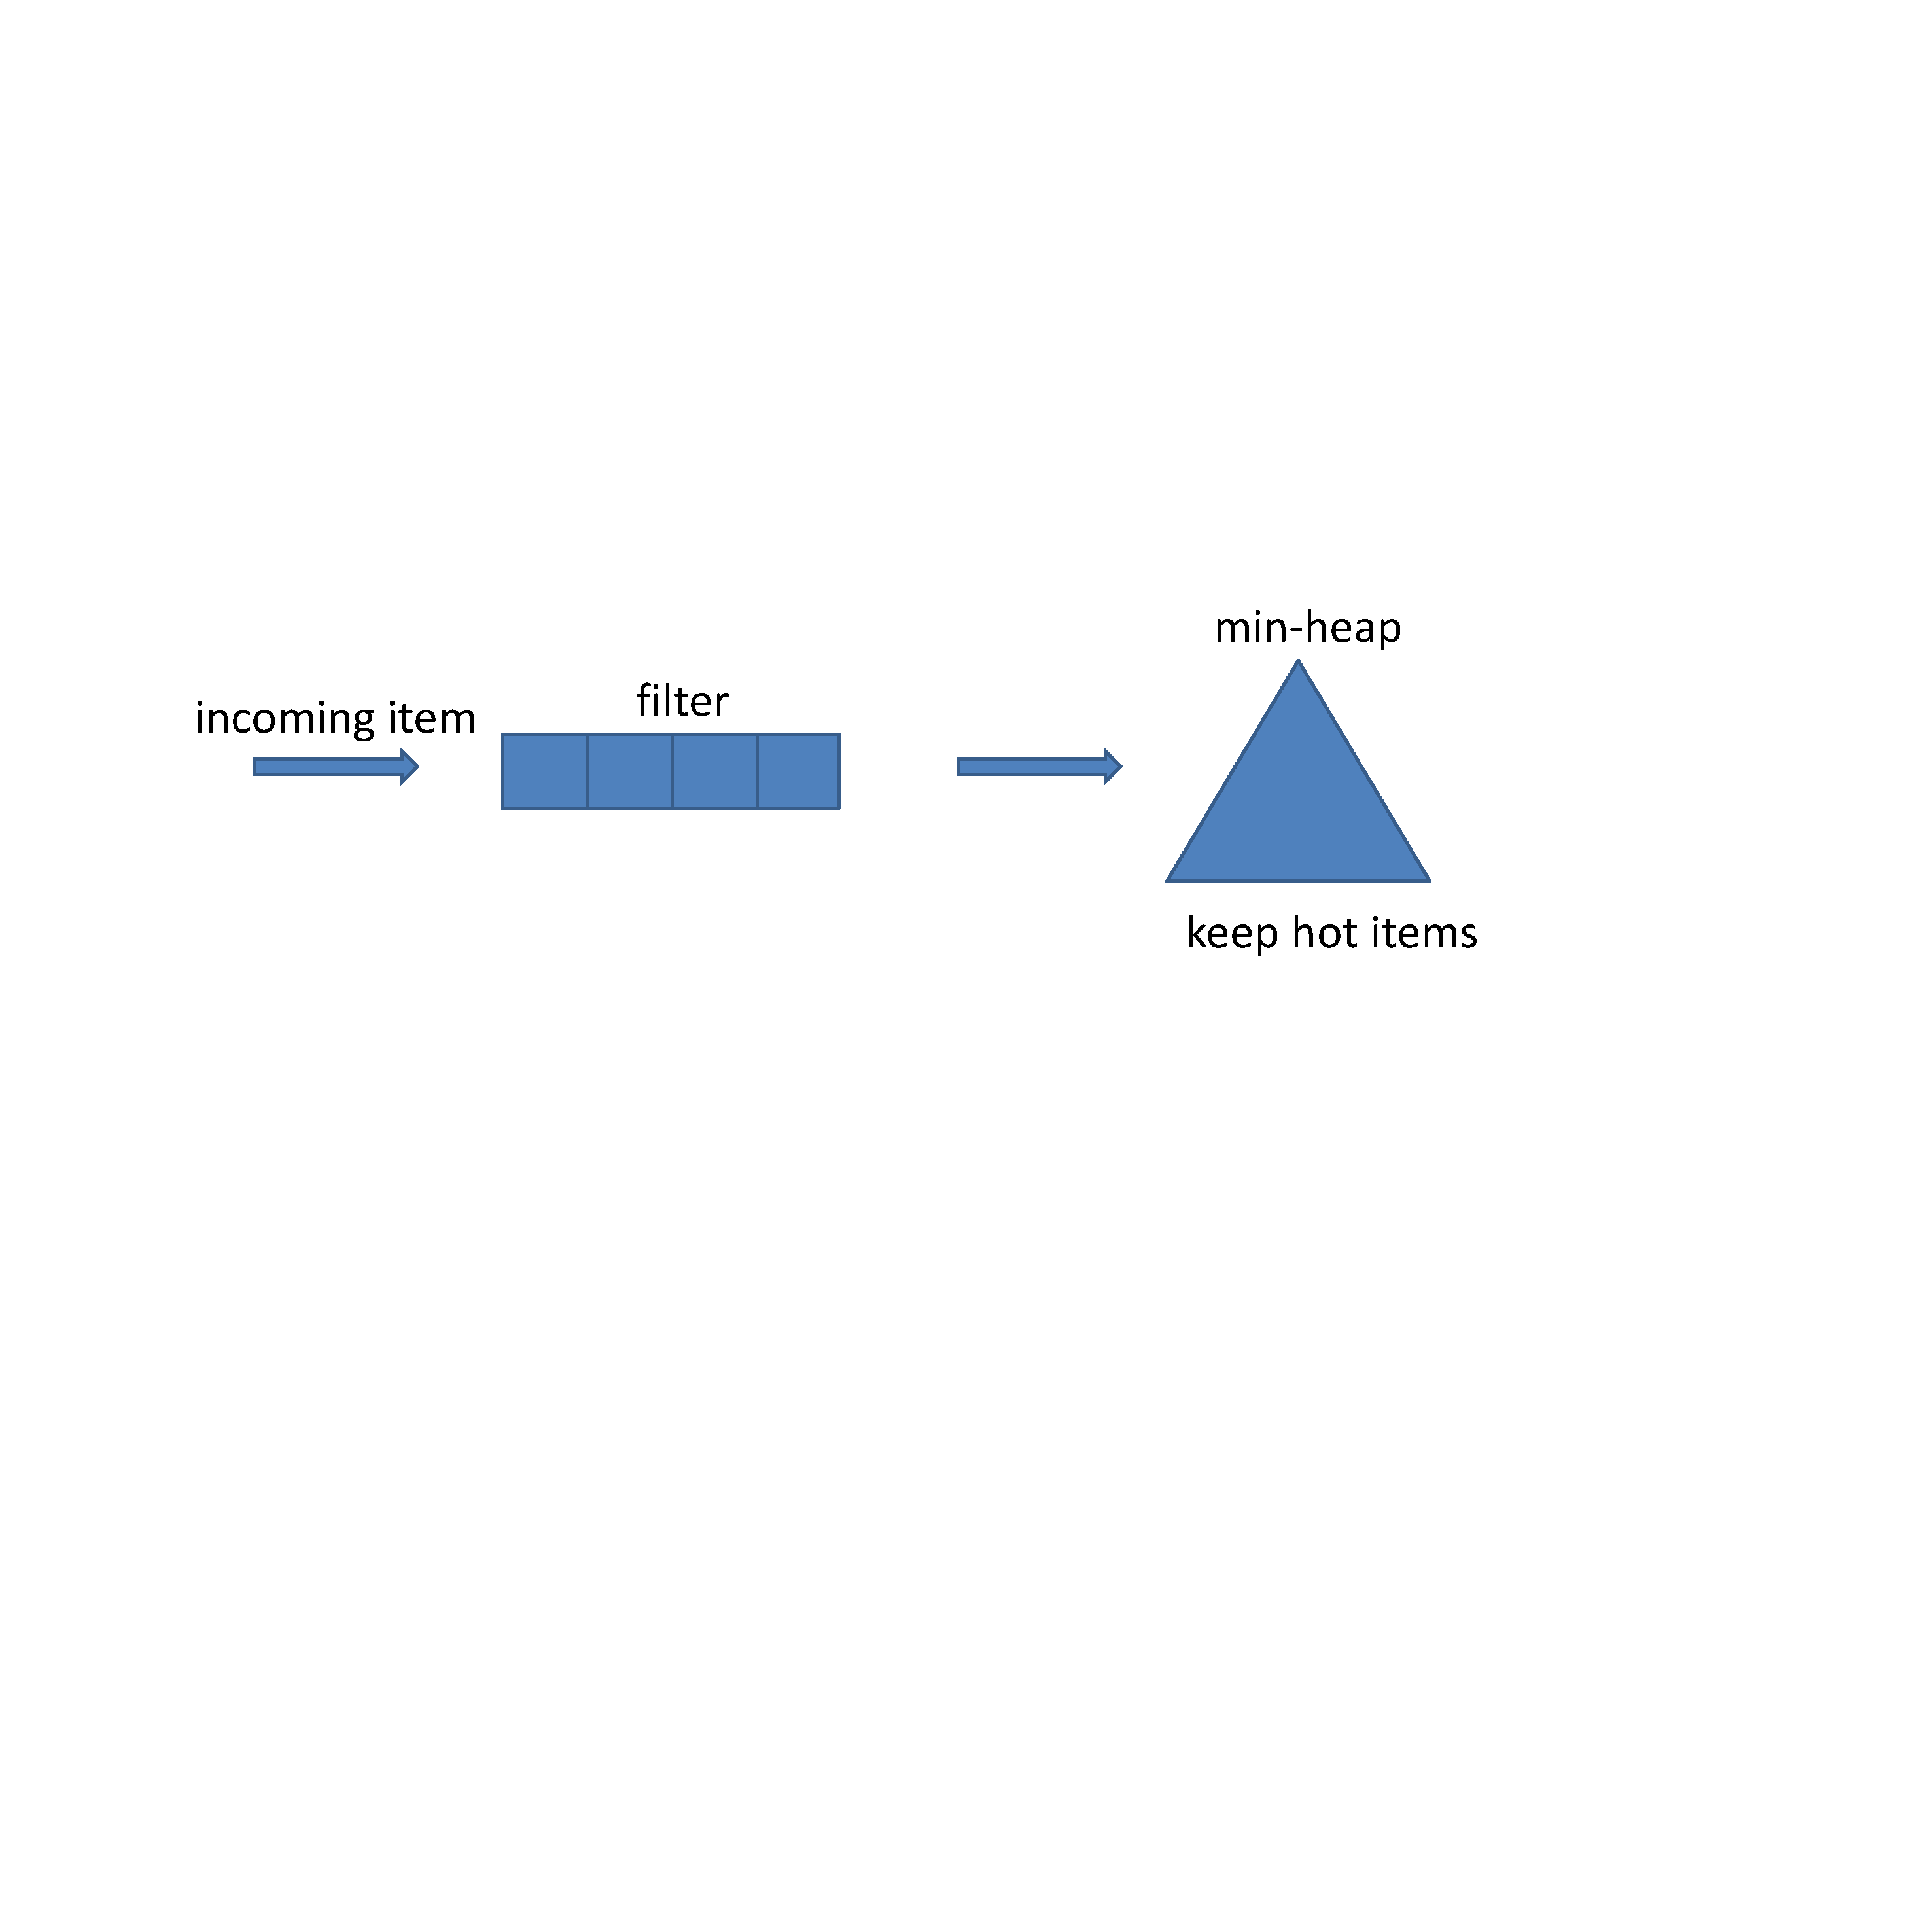
\includegraphics[width=0.45\textwidth]{framework}
	\prefigcaption \vspace{-0.05in} \vspace{-0.05in}
	\caption{The \aname{} framework.}
	\label{draw:interestframework}
	\postfig \vspace{-0.05in}
\end{figure}
%
To make our novelty clear, we first show the basic framework. It is simple: a filter (optional) and a min-heap. ``Optional'' means that some tasks do not need the filter.
%
Our key novelty is \textbf{\textit{the PRI technique}}.
%
In next Section (Section \ref{sec:optimization}), we will replace the min-heap to minimize the overhead of both time and space.

%achieve both memory efficiency and space efficiency.

\ppp{Data Structure (Figure \ref{draw:interestframework}):} 
The \aname{} framework consists of two parts. The first is a Bloom filter~\cite{BF1970}, used to remove duplicates in the incoming items. 
%
%Different definitions of interest has different operations of items in the Bloom filter. 
Duplicates removal is necessary because the interest \ii might not be incremented for every incoming item. For example, when finding persistent items, in each period, each incoming item can only increment the corresponding persistency by one, even though it might appear more than once in that period. 
%
The second part is a min-heap keeping hot items. In the min-heap, each node stores the information of an item, including item ID and interest \ii. The root node stores the item with the smallest interest. 

A Bloom filter~\cite{BF1970} is a compact data structure consisting of a number of bits and is often used when judging whether an item exists in a set or not. 
%
It is associated with $z$ hash functions.
%
There are mainly two operations for this data structure. 
%
The first is to insert an item $e$. 
%
The $z$ hash functions are first computed to pick out $z$ bits in the Bloom filter, and then all the $z$ bits are set to 1.
%
The second operation is to judge whether an item belongs to the set. The same $z$ hash functions are first computed to get the $z$ bits, and only if all the $z$ bits are 1, the Bloom filter reports true; otherwise, it reports false.
%
If the item is indeed in the set, true is always reported, \ie, it has no false negative error. 
%
In some cases, when an item does not belong to the set, the Bloom filter might also report true, which is called as false positive. However, the probability of false positive is often small enough to be acceptable in practice. 
%
Therefore, Bloom filters are used in various fields, especially in approximate data stream processing.


%%
\ppp{Insertion:}
Given an incoming item $e$, we first check the Bloom filter to judge whether $e$ is a duplicate: if the Bloom filter reports true, which means $e$ is a duplicate, and then $e$ is discarded. Otherwise, $e$ is inserted into the Bloom filter, and then we insert $e$ in the min-heap. There are two cases:

\textit{Case 1:} The item $e$ is in the min-heap. In this case, we increment the interest \ii{} by one.

\textit{Case 2:} $e$ is not in the min-heap. If the min-heap is not full, we insert $e$ into the min-heap. If the min-heap is full, we propose a technique named Probabilistic Replacement and then Increment (PRI for short) to \textit{probabilistically judge whether the incoming item is hot or cold.}

%%
\ppp{Probabilistic Replacement and then Increment (PRI):} This technique is the key novelty in this paper. Our PRI works as follows.
Suppose that the root node of the min-heap stores item $e_{min}$ with interest $\iii_{min}$.
Given an incoming item $e$ which is not in the min-heap, we replace $e_{min}$ with incoming item $e$ with a probability
%
$$\mathcal{P}=\frac{1}{2*\iii_{min}-
t_{fail}+1}$$
where $t_{fail}$ is the number of replacement failures.
%
If $e_{min}$ is successfully replaced by $e$, indicating that the interest of $e$ is likely to be larger than $e_{min}$, we increment the interest of $e_{min}$ from $\iii_{min}$ to $\iii_{min}+\lfloor t_{fail}/\iii_{min}\rfloor$ and set $t_{fail}$ to 0. 
%
Otherwise, $t_{fail}$ is incremented by 1.
%
For convenience, $\iii_{min}+\lfloor t_{fail}/\iii_{min}\rfloor$ is abbreviated to  $\iii_{min}+ t_{fail}/\iii_{min}$ in this paper.

{\color{reviewD}\hl{
\noindent\textbf{Designing the Expression of $\mathcal{P}$:}
We carefully design the expression of $\mathcal{P}$ to meet the following five properties. 
1) To successfully replace the original item, the value of $t_{fail}$ should reach an expectation of $\iii_{min}$.
%
2) The larger $\iii_{min}$ is, the less likely it is to be replaced.
3) The more replacement failures there are, the more likely the replacement will happen. 
4) When the number of replacement failures reaches $2*\iii_{min}$, the probability $\mathcal{P}$ increases to 1. This can avoid too many replacement failures.
5) When the replacement happens when number of replacement failures is small, $t_{fail}/\iii_{min}$ =0, we do not increase the smallest frequency. When the replacement happens when number of replacement failures is large, $t_{fail}/\iii_{min}$ =2, we increase the smallest frequency by 2. In other cases, we increase the smallest frequency by 0 or 1. 
}}


%
%We find that when the expression of $\mathcal{P}$ meets the above five properties, the accuracy is high and varies slightly.
%
%For example, we can use $\mathcal{P}=1/(3*\iii_{min}-t+1)$, or $i/(2*\iii)$, or.


%Analysis: In setting the probability of replacement, different probability leads to different accuracy. There are several alternatives: ({\color{red}$1/(\iii_{min}+1)$, $1/\iii_{min}$, $1/\iii_{min}^2$, $1/\lambda*\iii_{min}$, $1/2^{\iii_{min}}$, \textit{etc}.}) $1/(\iii_{min}+1)$, $1/\iii_{min}^2$, $1/(\lambda*\iii_{min})$, $1/c^{\iii_{min}}$, \textit{etc}. 
%Finally, we choose $1/(\iii_{min}+1)$ for two reasons. First, to successfully replace the original item, the number of new incoming items should reach an expectation of $\iii_{min}+1$.
%Second, the results of experiments show that the accuracy is the highest when the probability is  $1/(\iii_{min}+1)$ compared with all the other alternatives. 
%Otherwise, the interest $\iii_{min}$ remains unchanged.


%%
\ppp{Report:}
To report the items above a given threshold $\mathcal{T}$, we simply traverse the min-heap to return the items with interests larger than $\mathcal{T}$. 
%(see Algorithm \ref{alg:basic}).
\begin{comment}

Every time the interest of the item changes in the min-heap, we should adjust the min-heap. Therefore, we adjust the min-heap in lines $8^{th}$, $12^{th}$, and $18^{th}$.
%
Lines $14$ to $20$ of Algorithm \ref{alg:basic} are the implementation of the PRI technique.
%
Besides, in line $14$, we calculate the probability $\mathcal{P}$ by producing a random number between 0 and 1, because the probability that the random number is less than $\frac{1}{2*f_{min}-t_{fail}+1}$ is approximately equal to $\mathcal{P}$.
\end{comment}

\begin{comment}

\begin{algorithm}
	%	\SetLine
	\KwIn{An item $e_i$}
	$random()\in [0,1]$\\
	\eIf{$e_{i} \in$ Bloom\_filter}
	{
	    $return$\;
	}
	{
	$Bloom\_filter.insert(e_i)$\;
	\eIf{$e_{i} \in min\_heap$}
	{
		$Interest(e_{i})++$\;
		$min\_heap.adjust()$\;
	}
	  {
        \eIf{$min\_heap$ has empty buckets}
	        {
	        $min\_heap.insert(e_{i})$\;	
	        $min\_heap.adjust()$\;
	        }
	   {
	       \eIf{$random() \leqslant \frac{1}{2*\iii_{min}-
t_{fail}+1}$}
              {
	           $v_{min} \gets e_i$\;
	           $\iii_{min} \gets \iii_{min} + \frac{t_{fail}}{\iii_{min}}$\;
	           $t_{fail} \gets 0$\;
	           $min\_heap.adjust()$\;
	          }
	          {
	          $t_{fail}++$\;
	          }
	   }
	  }
	}
	\caption{Insertion process of InterestSketch.}
	\label{alg:basic}
\end{algorithm}
\end{comment}

%
\begin{figure}[htbp]
	\centering
	\prefig
	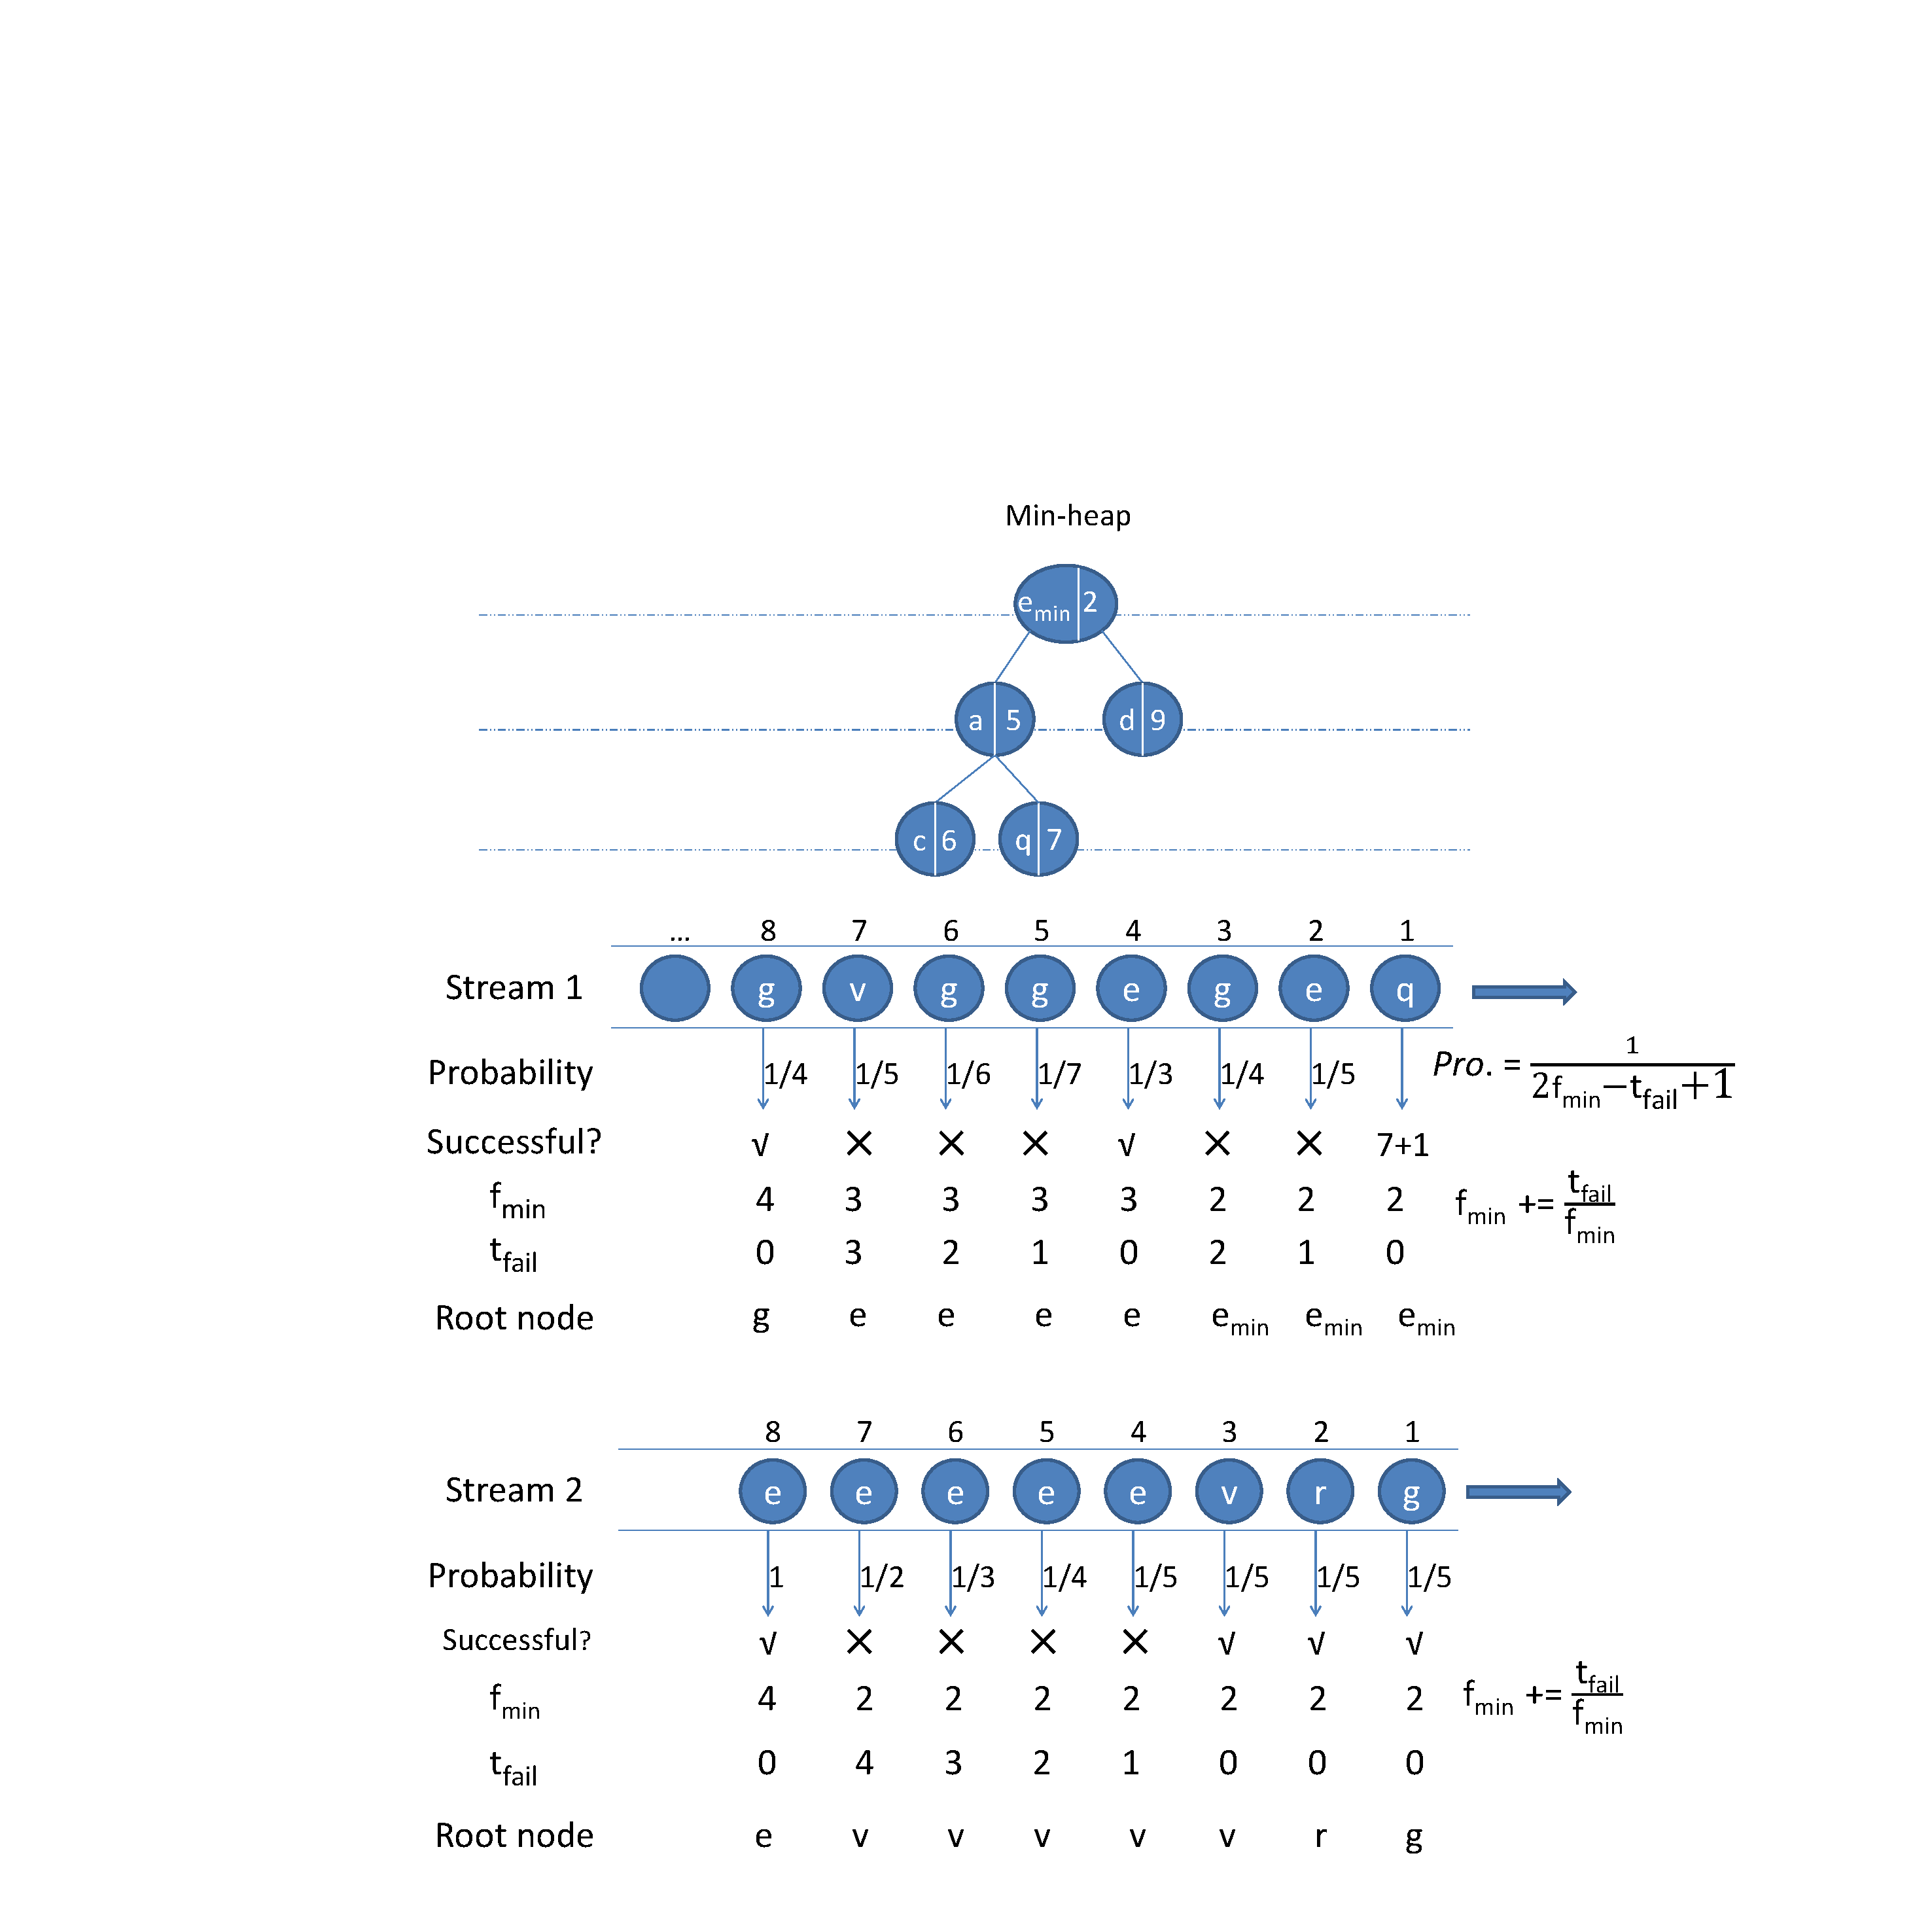
\includegraphics[width=0.5\textwidth]{GraphPPT/example_freq}
	\prefigcaption \vvv\vvv
	\caption{\hl{Examples of PRI when Interest is frequency.}
    }
	\label{draw:freq}
	\postfig \vvv\vvv
\end{figure}
%

\hl{
To clearly show the advantage of PRI, we give two common running examples to show how PRI works. 
Without loss of generality, in these two examples, we let frequency be the interest of items.}
%
\hl{
\mbox{\noindent\textbf{Example 1 (Figure~\ref{draw:freq}):}}
Given a data stream (stream 1): $q,e,g,e,g,g,v,g$, for the first incoming item $q$, we increment the frequency of $q$ in the min-heap by one.
For the following two items $e$ and $g$, replacements fail, and thus $t_{fail}$ is incremented to 1 and then 2. 
The probability increases to 1/3 for the fourth item $e$.
Then $e_{min}$ is successfully replaced by the fourth item $e$ in the root node, and the frequency $f_{min}$ is incremented by $\frac{t_{fail}}{f_{min}}=1$, from 2 to 3, and  $t_{fail}$ is reset to 0.
Since the actual frequency of item $e$ is 2 at present but we record it as 3, the frequency is slightly overestimated.
Then the following 3 items ($g$, $g$, $v$) arrive and replace $e$ with probabilities 1/7, 1/6, and 1/5, but all fail. 
Finally, the eighth item $g$ successfully replaces $e$ and the frequency $f_{min}$ is incremented from 3 to 4, which is exactly the frequency of item $g$ by now in data stream 1. }

\noindent\textbf{\hl{Example 2 (Figure} \ref{draw:freq}):}\hl{
Given another data stream (stream 2): $g, r, v, e, e, e, e, e$, suppose that each of the first three items successfully replaces the root node with the same probability of 1/5, and increments the frequency $f_{min}$ by $\frac{t_{fail}}{f_{min}}(=0)$ each time. 
%
Then item $e$ arrives five times in succession. 
After four unsuccessful replacements with probabilities 1/5, 1/4, 1/3, and 1/2, the eighth item $e$ replaces item $v$ in the root node with probability 1, and increments the frequency $f_{min}$ by $\frac{t_{fail}}{f_{min}}(=2)$, from 2 to 4. 
The frequency $f_{min}$ is slightly underestimated, since item $e$ has appeared 5 times in the data stream by now. 
The first three replacements are wrong, but do not bring a large error to the final value of $f_{min}$. }

\hl{
From the two examples, we see that in our algorithm, the frequency $f_{min}$ might be overestimated or underestimated.
Fortunately, an item might be overestimated at first, but it could be underestimated later, and finally the estimate of the item is probably very close to its true value.
Moreover, successful replacement of infrequent items hardly impact the final result of $f_{min}$.
}

%\xy{$t_{fail}$ of the last e should be 0}

Next, we apply our framework to four specific problems in the following sections.
{
\color{reviewD}
For each problem, we describe the data structure, insertion, and report. Note that we focus only on the variations across the approaches in the specific subsections.
%variation of each problem from the InterestSketch framework.
}


